%%%%%%%%%%%%%%%%%%%%%%%%%%%%%%%%%%%%%%%%%
% Journal Article
% LaTeX Template
% Version 1.4 (15/5/16)
%
% This template has been downloaded from:
% http://www.LaTeXTemplates.com
%
% Original author:
% Frits Wenneker (http://www.howtotex.com) with extensive modifications by
% Vel (vel@LaTeXTemplates.com)
%
% License:
% CC BY-NC-SA 3.0 (http://creativecommons.org/licenses/by-nc-sa/3.0/)
%
%%%%%%%%%%%%%%%%%%%%%%%%%%%%%%%%%%%%%%%%%

%----------------------------------------------------------------------------------------
%	PACKAGES AND OTHER DOCUMENT CONFIGURATIONS
%----------------------------------------------------------------------------------------

\documentclass[twoside,twocolumn]{article}

\usepackage{blindtext} % Package to generate dummy text throughout this template 

\usepackage[sc]{mathpazo} % Use the Palatino font
\usepackage[T1]{fontenc} % Use 8-bit encoding that has 256 glyphs
\linespread{1.05} % Line spacing - Palatino needs more space between lines
\usepackage{microtype} % Slightly tweak font spacing for aesthetics

\usepackage[english]{babel} % Language hyphenation and typographical rules

\usepackage[hmarginratio=1:1,top=32mm,columnsep=20pt]{geometry} % Document margins
\usepackage[hang, small,labelfont=bf,up,textfont=it,up]{caption} % Custom captions under/above floats in tables or figures
\usepackage{booktabs} % Horizontal rules in tables

\usepackage{lettrine} % The lettrine is the first enlarged letter at the beginning of the text

\usepackage{enumitem} % Customized lists
\setlist[itemize]{noitemsep} % Make itemize lists more compact

\usepackage{abstract} % Allows abstract customization
\renewcommand{\abstractnamefont}{\normalfont\bfseries} % Set the "Abstract" text to bold
\renewcommand{\abstracttextfont}{\normalfont\small\itshape} % Set the abstract itself to small italic text

\usepackage{titlesec} % Allows customization of titles
\renewcommand\thesection{\Roman{section}} % Roman numerals for the sections
\renewcommand\thesubsection{\roman{subsection}} % roman numerals for subsections
\titleformat{\section}[block]{\large\scshape\centering}{\thesection.}{1em}{} % Change the look of the section titles
\titleformat{\subsection}[block]{\large}{\thesubsection.}{1em}{} % Change the look of the section titles

\usepackage{fancyhdr} % Headers and footers
\pagestyle{fancy} % All pages have headers and footers
\fancyhead{} % Blank out the default header
\fancyfoot{} % Blank out the default footer
\fancyhead[C]{IBMQ App $-$ Jan 2019 $-$ IBM Q Italy} % Custom header text
\fancyfoot[RO,LE]{\thepage} % Custom footer text

\usepackage{titling} % Customizing the title section
\usepackage{graphicx} % Add images
\usepackage{hyperref} % For hyperlinks in the PDF
\usepackage{lscape} % For rotating tables
\usepackage{subcaption} % For subfigures

\graphicspath{{img/}}
%----------------------------------------------------------------------------------------
%	TITLE SECTION
%----------------------------------------------------------------------------------------

\setlength{\droptitle}{-4\baselineskip} % Move the title up

\pretitle{\begin{center}\Huge\bfseries} % Article title formatting
\posttitle{\end{center}} % Article title closing formatting
\title{IBMQ App\\A testing framework for real quantum computing usage} % Article title
\author{%
\textsc{F. Accetta} \and \textsc{G. Agliardi} \and \textsc{A. Aita} \and
\textsc{L. Crippa} \and \textsc{M. Grossi} \and \textsc{F. Tramonto} \\
%\and % Uncomment if 2 authors are required, duplicate these 4 lines if more
%\textsc{Jane Smith}%\thanks{Corresponding author} \\[1ex] % Second author's name
%\normalsize University of Utah \\ % Second author's institution
%\normalsize \href{mailto:jane@smith.com}{jane@smith.com} % Second author's email address
}
%\date{\today} % Leave empty to omit a date
\date{January 31, 2019} % Leave empty to omit a date
\renewcommand{\maketitlehookd}{%
\begin{abstract}
\noindent 
\lettrine[nindent=0em,lines=3]{G}enerally the learning process follow some specific and pedagocic steps. Sometimes we need to be caputered by a new technology to gather its power and if we are able to give the reader a visual and intuitive explanation of difficult concept we can make the difference.
The growing importance of quantum computing can be exploited where the backend engine is not working with bits but with their quantum version. In this paper we describe a three Tier web application deployed on IBM Cloud. We propose visual representation for explaining single qubit gate effect and the quantum version of the so called Hello World code.
This web APP is thought as an alternative to jupyter notebooks approach and can be easily shared (public URL and login).

\end{abstract}
}

%----------------------------------------------------------------------------------------

\begin{document}

% Print the title
\maketitle

%----------------------------------------------------------------------------------------
%	ARTICLE CONTENTS
%----------------------------------------------------------------------------------------




\section{Algorithm description}\label{cap:science}

%Text requiring further explanation\footnote{Example footnote}.

\subsection{Generalized quantum emoticon}
Anything that can be done with bits can be done with qubits. Simply leave a qubit in its initialized value for the state $0$, or use an operation with the effect of a NOT gate (such as X or Y) to rotate it to a $1$. Each qubit then becomes a bit, allowing us to implement Hello, World! directly on a quantum computer.

In practice, it is not so straightforward. ASCII encoding of Hello, World! requires over $100$ bits, and therefore over $100$ qubits. Current quantum devices are not yet large enough for the job.

In this application we propose a generalization of what is presented on IBMQ Experience tutorial (\href{
https://github.com/Qiskit/qiskit-tutorials/blob/master/community/hello_world/quantum_emoticon.ipynb
}{Quantum Emoticon} where the reader can test how the two main principles of quantum computing are exploited: the superposition and the entanglement. Here the reader can use every combination of ASCII character and visualize their realization with qubits, either simulated or real according to what is available on IBMQ Experience.


For more information about how to use the IBM Q ExperienceQX, consult the \href{https://quantumexperience.ng.bluemix.net/qstage/#/tutorial?sectionId=c59b3710b928891a1420190148a72cce&pageIndex=0}{tutorials}, or check out the \href{https://quantumexperience.ng.bluemix.net/qstage/#/community}{community}.

\subsection{Bloch Sphere's representation}

This APP feature make use of well known math representation of vector in $3$ dimension which is widely used in this quantum computing dissemination as it is a clear and and usefull tool: the Bloch Sphere.
The user can visualize the effect of quatum gate application on its qubit (versor). Since we are working with orthonormal basis we give the user the freedom to star from different basis: X-basis, Y-basis or Z-basis. Current version of the application does not allow subsequent gate application so the user must reset its result before applying a new transformation.
The user can perform measurement of the quantum state on all the three basis (x,y,z)
in order to reconstruct the quantum state on the Bloch Sphere. In order to make this algorithm fully visual we utilized the python library qutip that allows
to perform analytical calculation and build the block sphere.

The interesting feature is that the result of gate application is showed on two separate Bloch Spheres. In the left one the user is presented the result coming from IBMQ Experience while on the right one we present the analytic result. This comparison can help to understand some typical quantum defects coming from real hardware noise or approximation.


This algorithm it's defined inside the ibm quantum experience User guide, it consist to 
We decided to offer two different prospectives giving two bloch-spheres, one to show the QST performance and another one to show the analytical calculation, in order to
give evidence of the errors coming from dechoerence/noise generated from the real device or from the configured noise-simulator.


\href{https://quantumexperience.ng.bluemix.net/proxy/tutorial/full-user-guide/002-The_Weird_and_Wonderful_World_of_the_Qubit/005-The_Bloch_Sphere.html}{Spheres}

\href{https://en.wikipedia.org/wiki/Quantum_tomography}{Quantum Tomography}


\section{Architecture representation}
In this section we describe the overall application architecture. 

\begin{center}
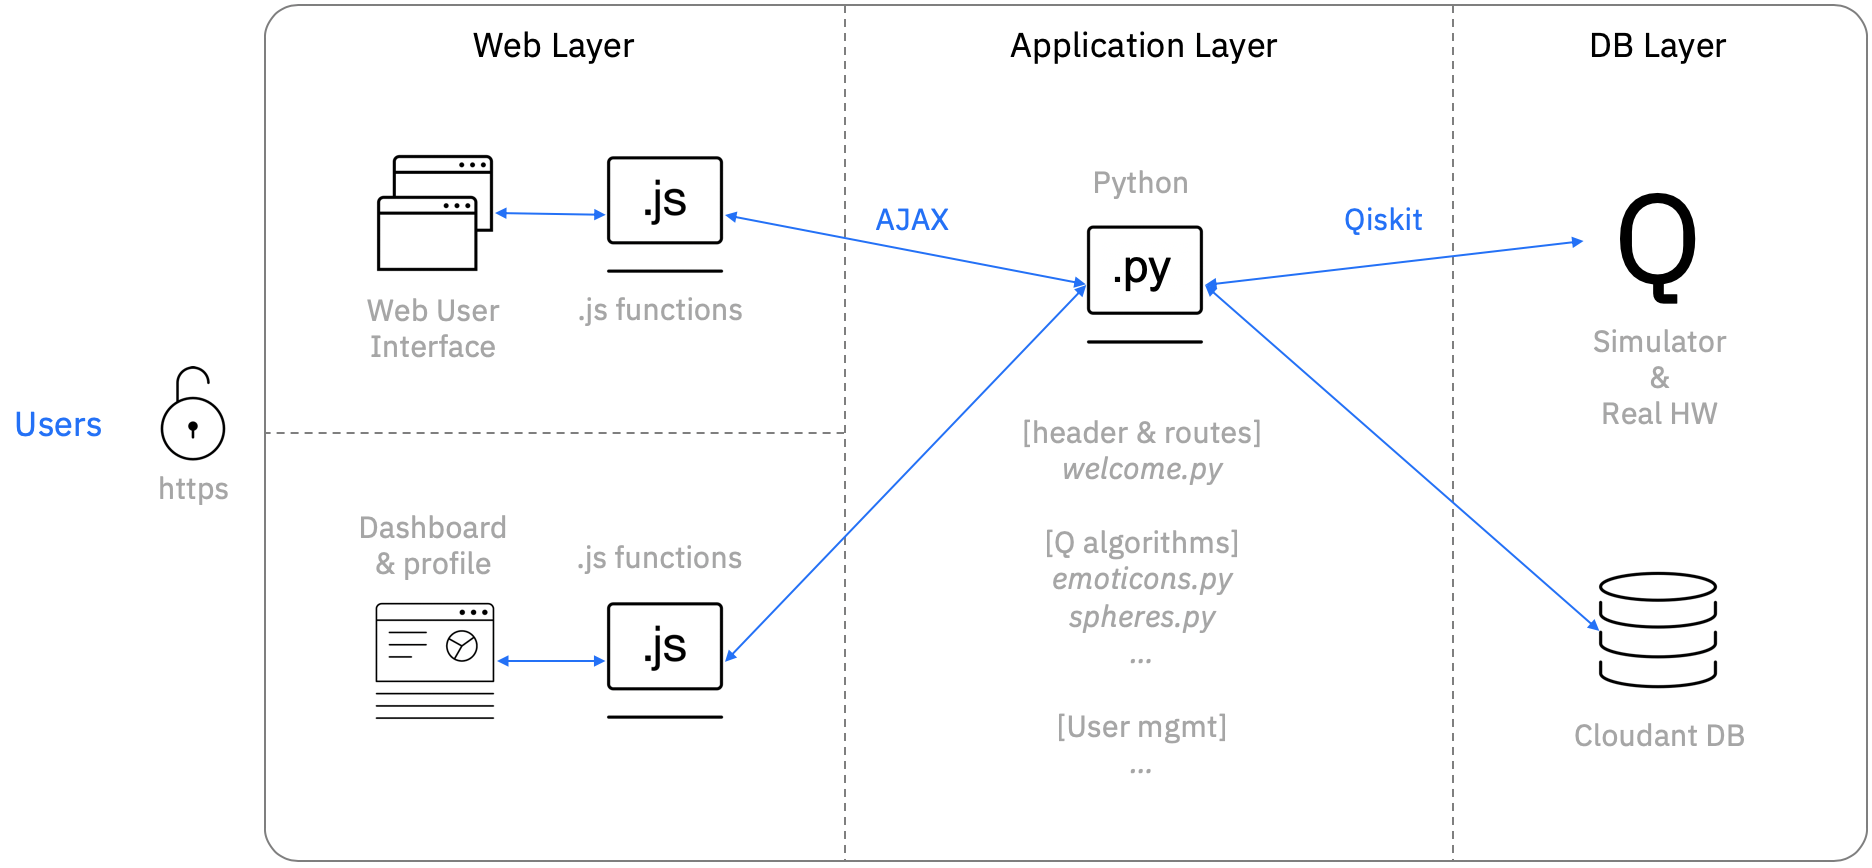
\includegraphics[scale=0.4]{architecture.png}
\end{center}

\begin{center}
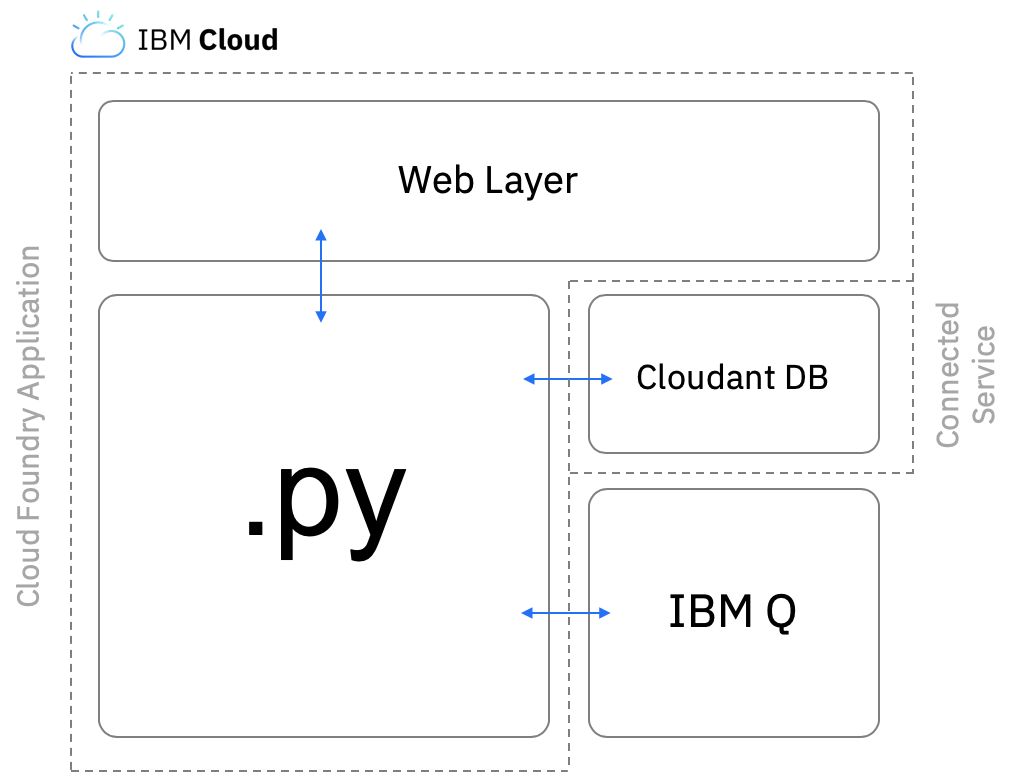
\includegraphics[scale=0.4]{hl_architecture.png}
\end{center}

%------------------------------------------------

\section{Conclusions}

We are happy.



%------------------------------------------------


%----------------------------------------------------------------------------------------
%	REFERENCE LIST
%----------------------------------------------------------------------------------------

\begin{thebibliography}{99}

\bibitem{chuang}
Hand, D. J. (n.d.).,
{\it Measuring classifier performance: A coherent alternative to the area under the ROC curve.}%\url{http://arxiv.org/abs/1303.5062}.

\end{thebibliography}

%----------------------------------------------------------------------------------------

\end{document}
